\begin{figure}
\begin{adjustbox}{minipage=1.0\linewidth,frame}
\vspace{2.5mm}
\centering

\begin{subfigure}[t]{.45\linewidth}
    \centering
    \captionsetup[subfigure]{}
    \caption{3-day readmission.}\label{fig:shaprdt3d}
    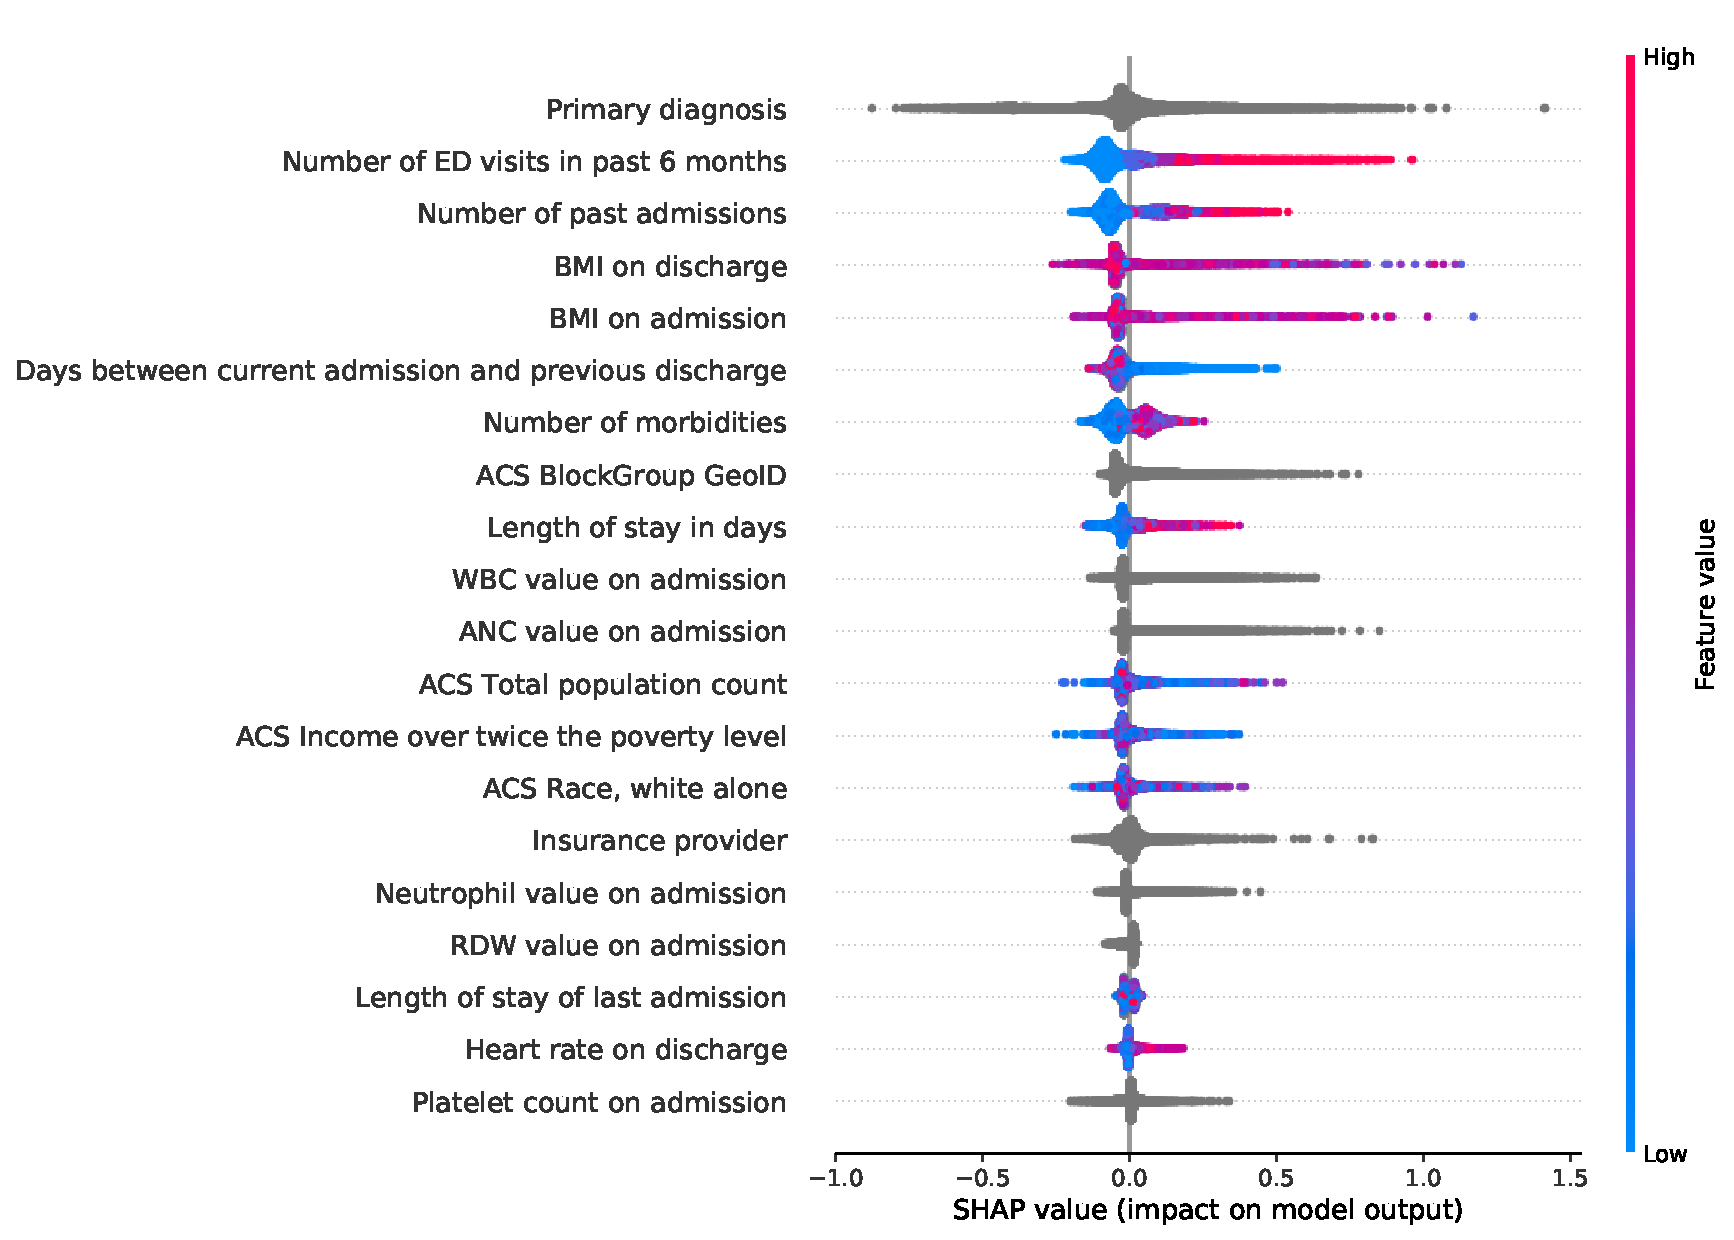
\includegraphics[width=\linewidth,keepaspectratio]{supplementary/readmitted3d_SHAP_summary.pdf}
\end{subfigure}%
\begin{subfigure}[t]{.45\linewidth}
    \centering
    \captionsetup[subfigure]{}
    \caption{7-day readmission.}\label{fig:shaprdt7d}
    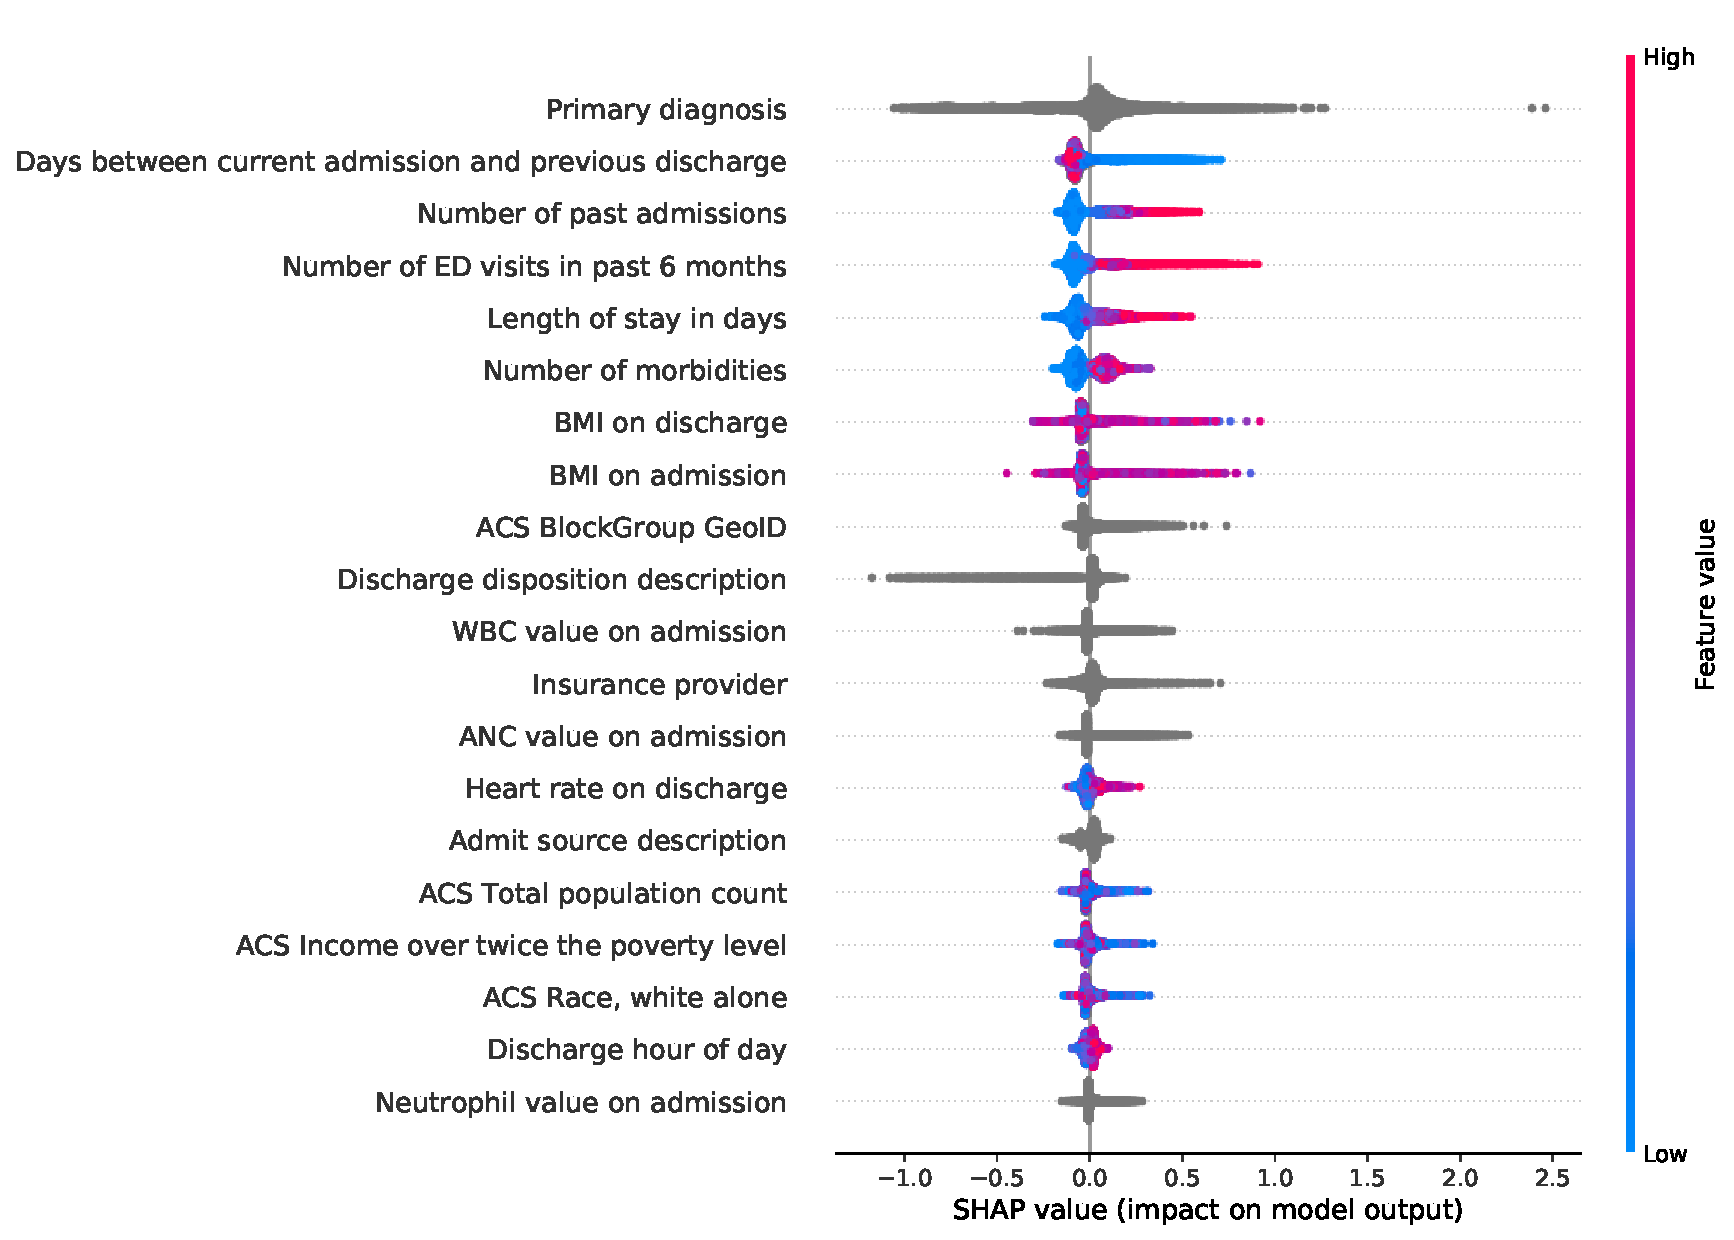
\includegraphics[width=\linewidth,keepaspectratio]{supplementary/readmitted7d_SHAP_summary.pdf}
\end{subfigure}%

\begin{subfigure}[t]{.45\linewidth}
    \centering
    \captionsetup[subfigure]{}
    \caption{Length of stay over 3 days.}\label{fig:shaplos3d}
    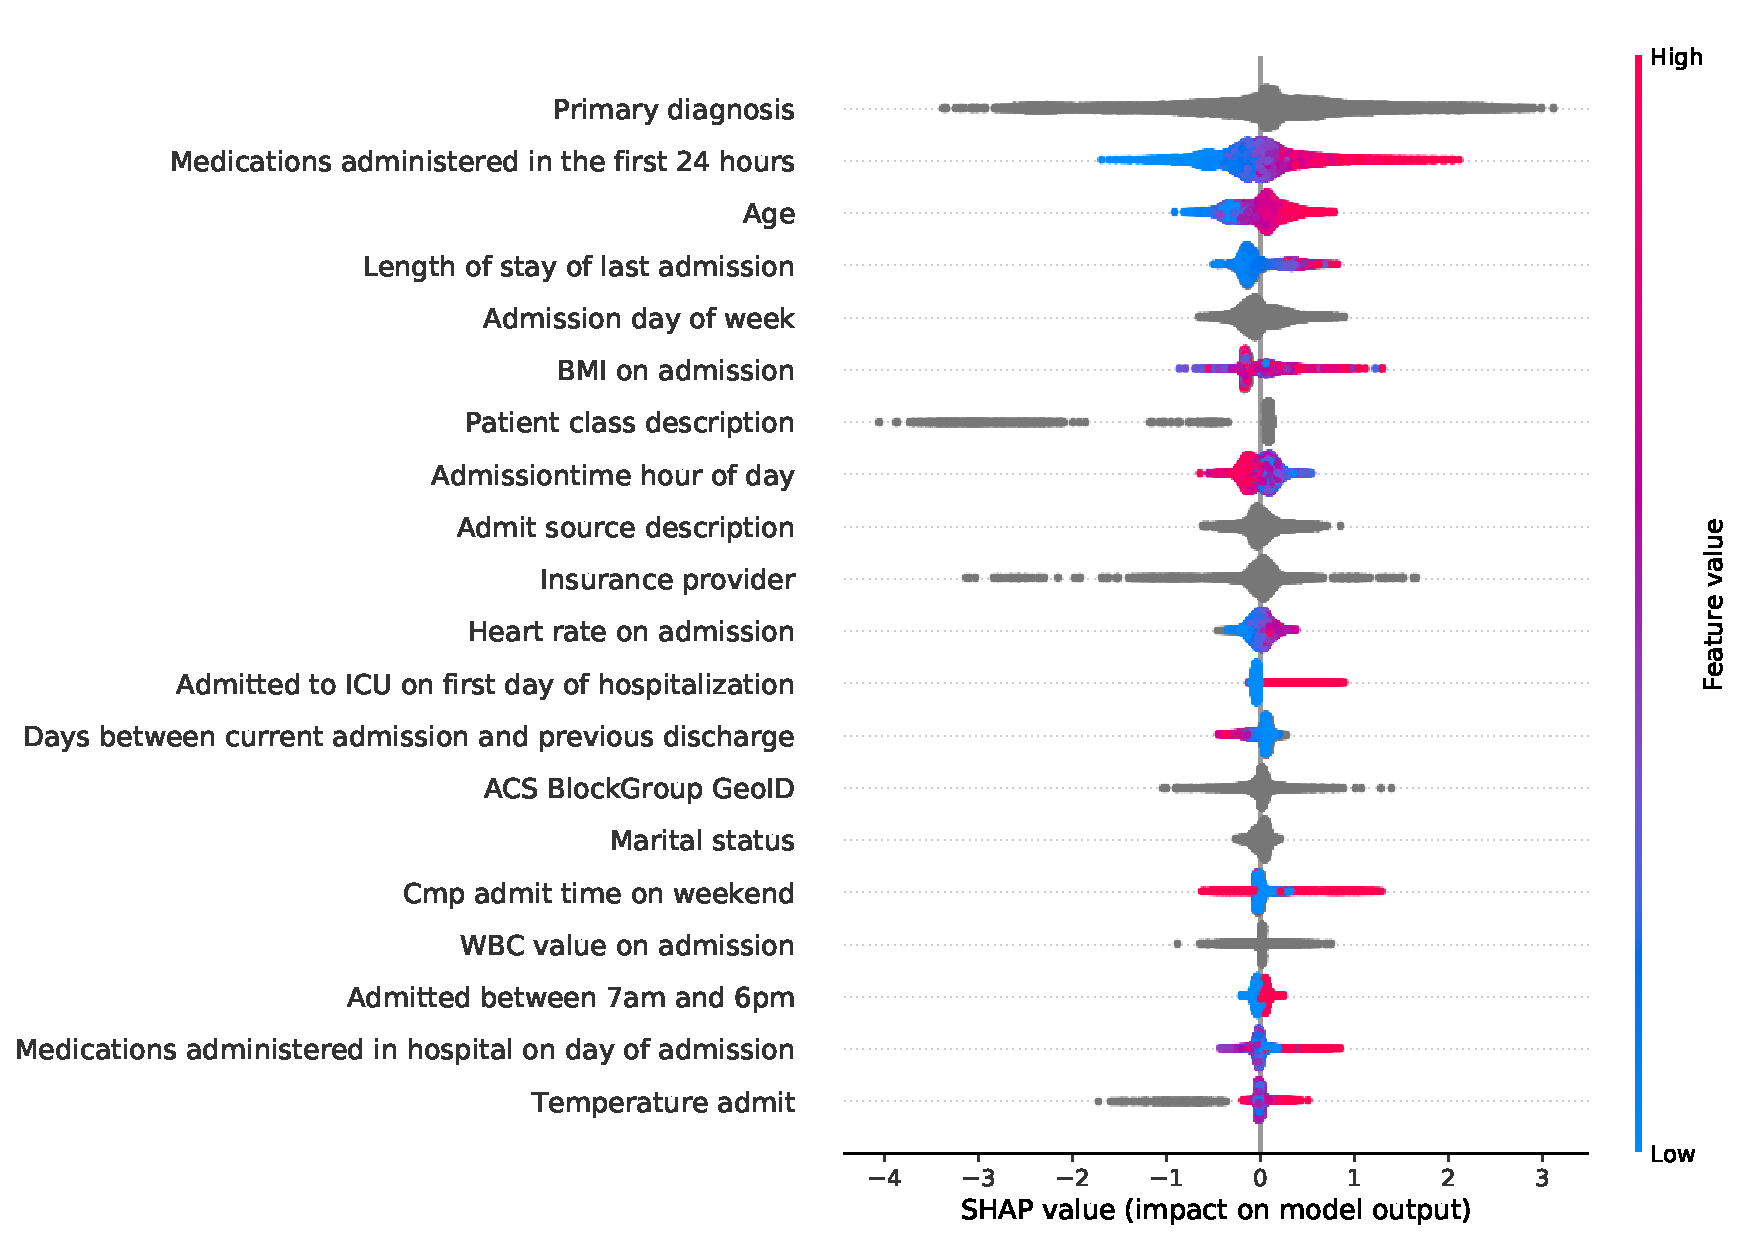
\includegraphics[width=\linewidth,keepaspectratio]{supplementary/los3d_SHAP_summary.pdf}
\end{subfigure}%
\begin{subfigure}[t]{.45\linewidth}
    \centering
    \captionsetup[subfigure]{}
    \caption{Length of stay over 3 days.}\label{fig:shaplos7d}
    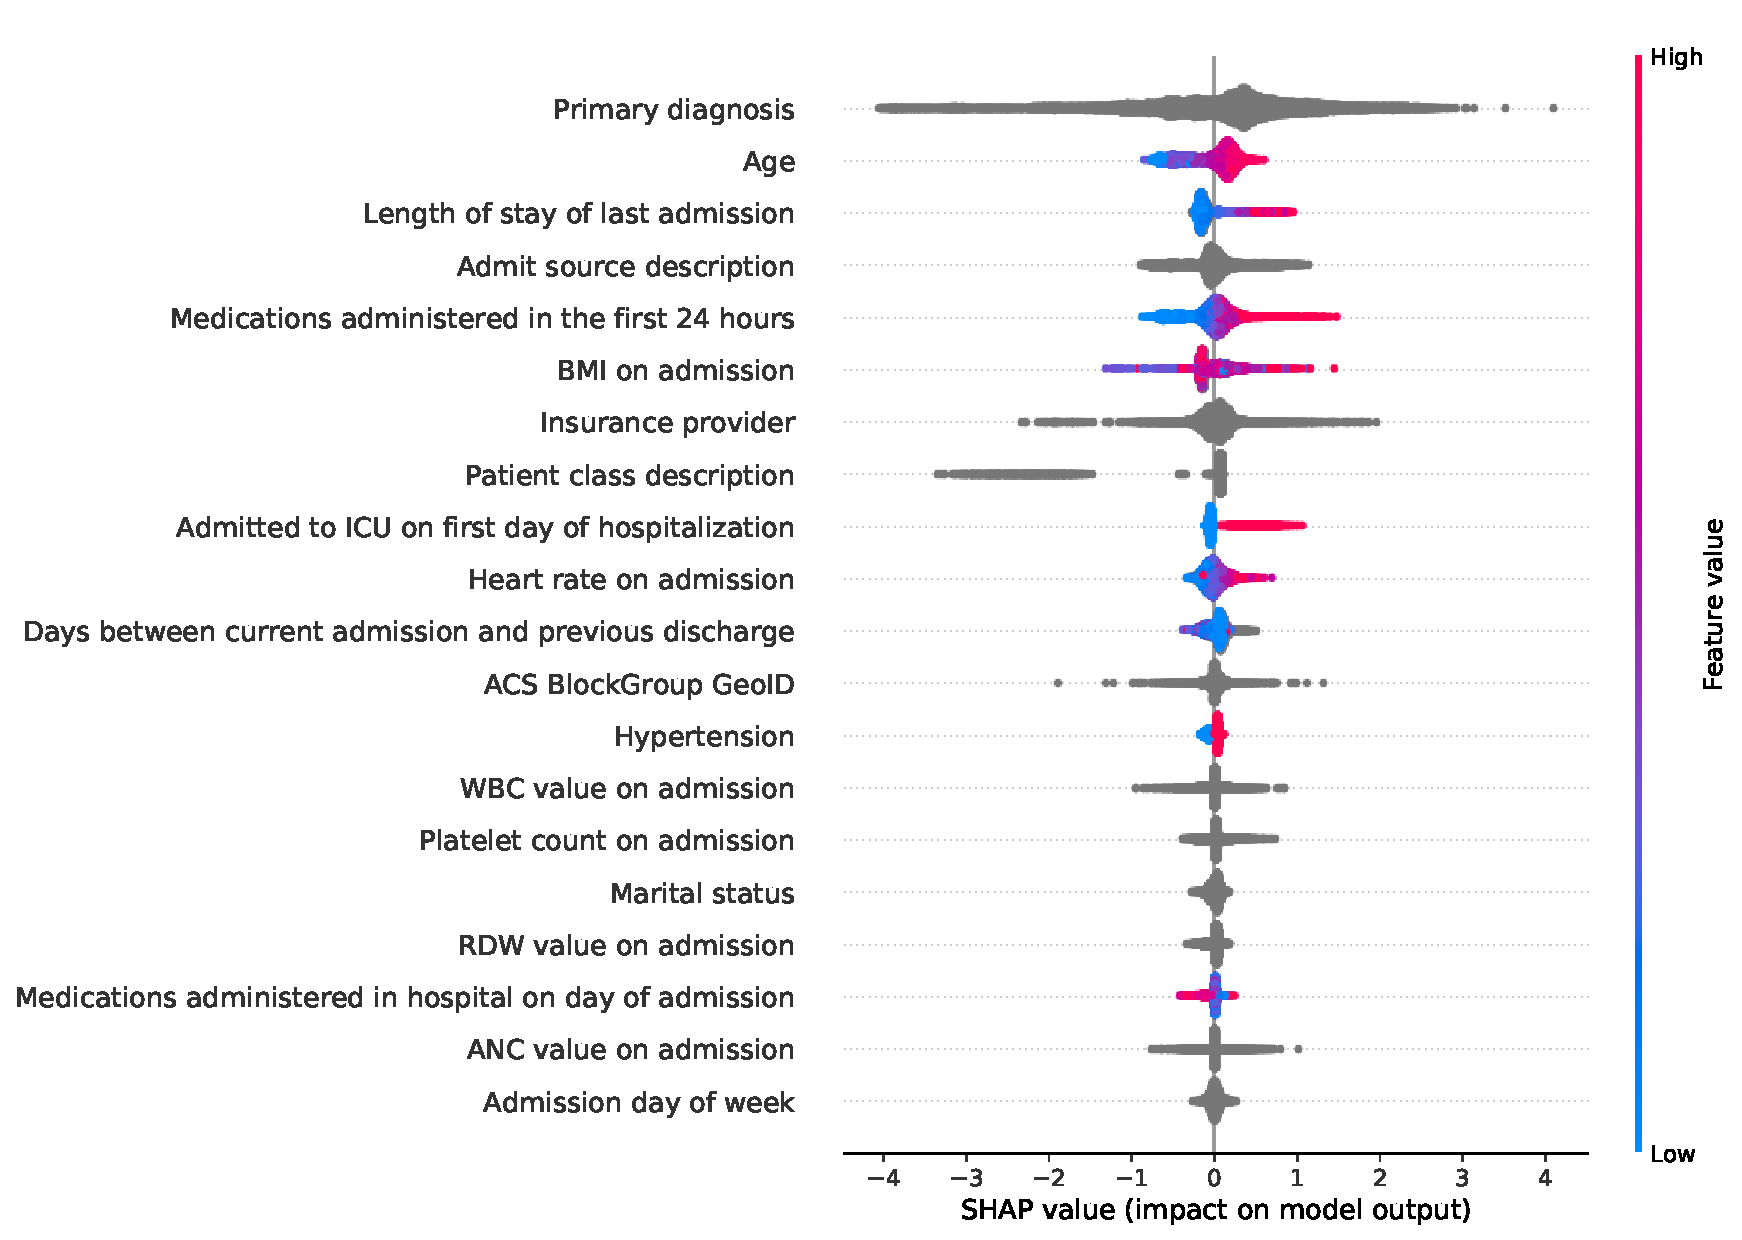
\includegraphics[width=\linewidth,keepaspectratio]{supplementary/los7d_SHAP_summary.pdf}
\end{subfigure}%

\caption{\textbf{Prediction of Hospitalization Outcomes.} \\
Panels~\ref{fig:shaprdt3d},~\ref{fig:shaprdt7d},~\ref{fig:shaplos3d}, and~\ref{fig:shaplos7d} 
show the most impactful features on prediction, 
along with the impact of high or low values for numeric features. Categorical features are shown in gray.\@
}\label{fig:suppshapfig}
\end{adjustbox}
\end{figure}